
\input{chapters/template.tex}

\begin{document}

\frontmatter

\newgeometry{
    top=24mm,
    bottom=28mm,
    left=39mm,
    right=39mm,
    heightrounded
}
\begin{titlepage}
    \centering

    \makebox[\textwidth][c]{\Huge\bfseries Fisica 3 \par}

    \vspace{1cm}

    \makebox[\textwidth][c]{\Large Roberto Riccucci \par}

    \vspace{1.5cm}

    \makebox[\textwidth][c]{\rule{0.8\textwidth}{0.4pt}}

    \vspace{0.7cm}

    \makebox[\textwidth][c]{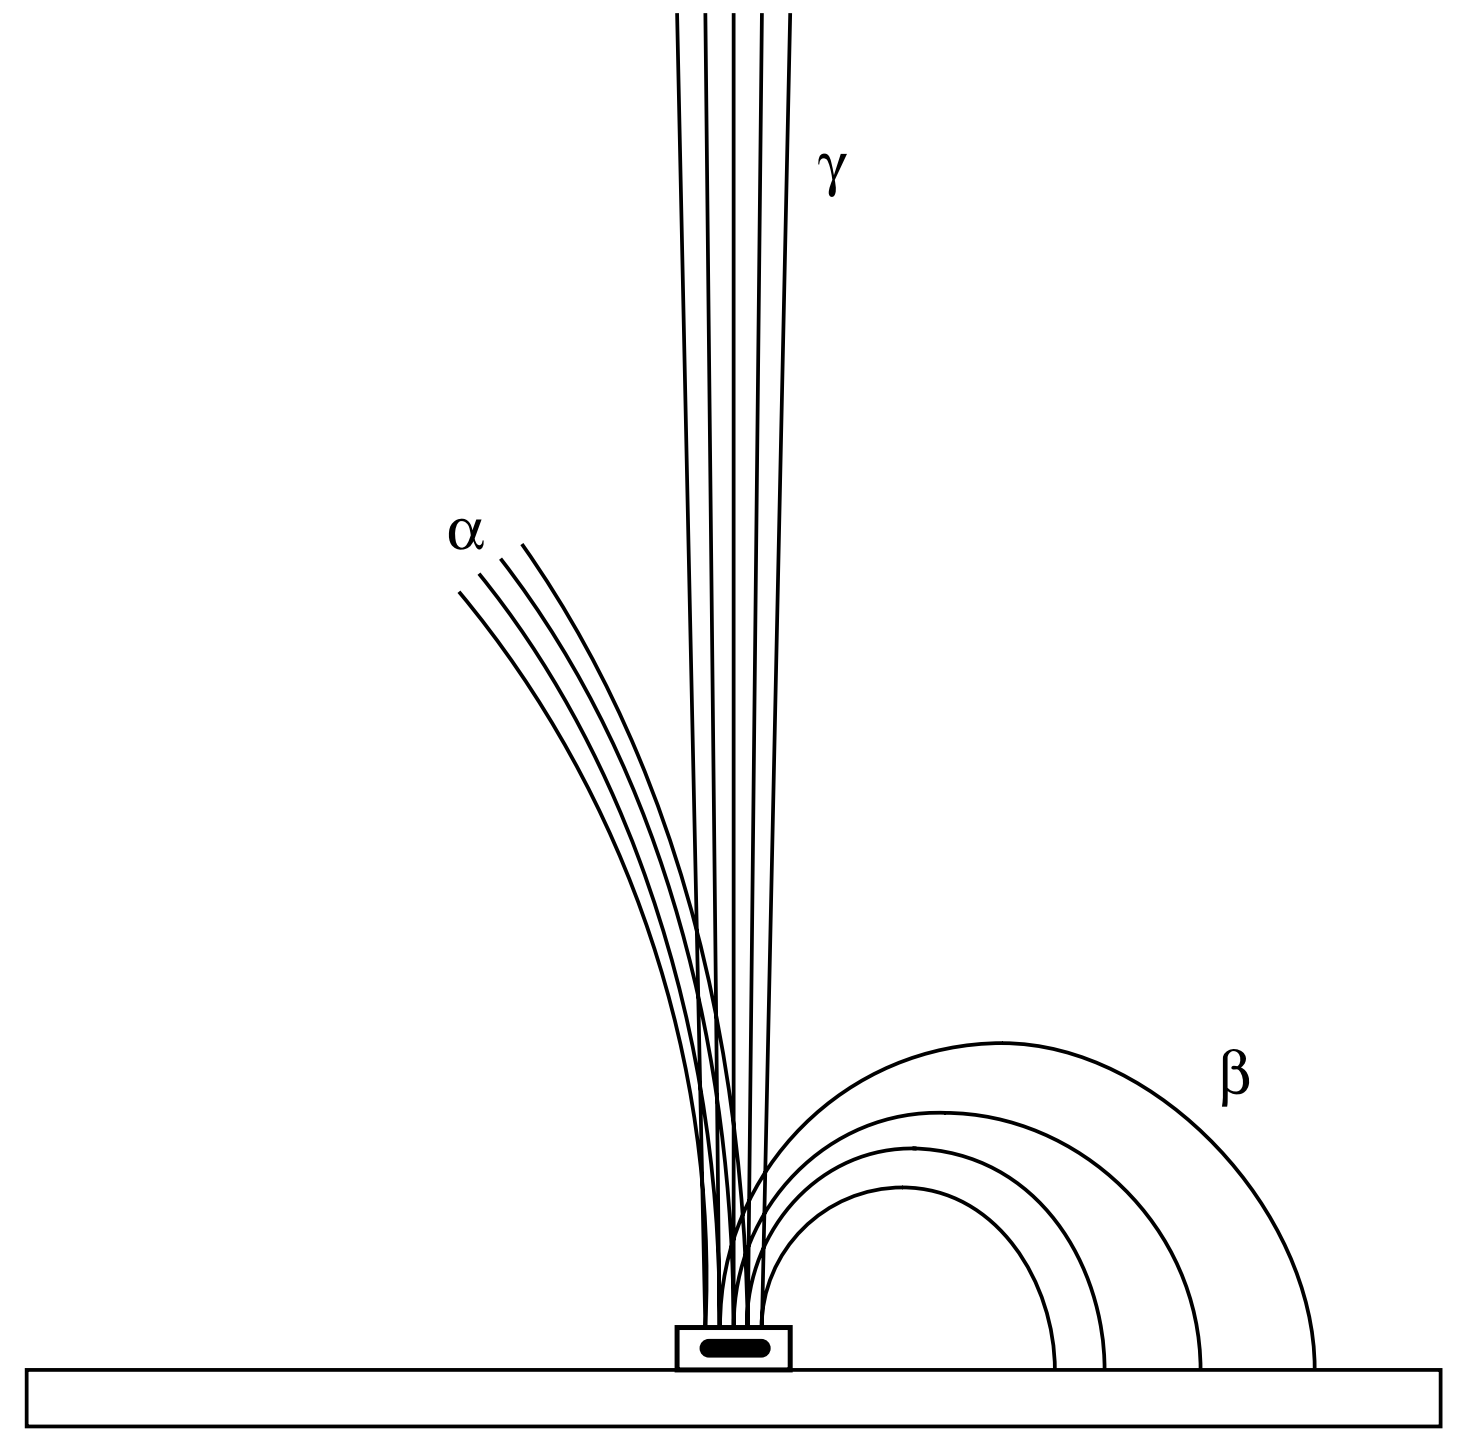
\includegraphics[width=0.7\textwidth]{foto/particelle.png}}

    \vspace{0.7cm}

    \makebox[\textwidth][c]{\rule{0.8\textwidth}{0.4pt}}

    \vfill

    \makebox[\textwidth][c]{\large Versione v0.1 \par}
    \makebox[\textwidth][c]{\small robertoriccucci1304@gmail.com \par}

\end{titlepage}
\restoregeometry

\addchap{Prefazione}

Questi appunti, insieme al codice \LaTeX{} e a tutte le immagini, sono disponibili sulla mia pagina GitHub: \url{https://github.com/RobertoRiccucci/Appunti-Fisica-3}

\begin{flushright}
Roberto Riccucci\\
Pisa, \today
\end{flushright}


\tableofcontents

\mainmatter

% --- Teoria ---

\newgeometry{
    a4paper,
    top=24mm,
    bottom=28mm,
    left=39mm,
    right=39mm,
    heightrounded
}
\partpage{Teoria}
\restoregeometry


\chapter{Decadimenti}

La fisica nucleare ha avuto un ruolo centrale nello sviluppo della fisica del $20^\circ$ secolo, sia sul piano teorico sia su quello sperimentale. 
Pochi altri campi scientifici abbracciano uno spettro di fenomeni così vasto: gli esperimenti di fisica nucleare hanno contribuito a comprendere processi che vanno dalle interazioni tra i quark, i costituenti più elementari della materia, fino a quanto avvenuto nelle prime fasi dell'universo, subito dopo il Big Bang. 
Anche le sue tecniche hanno trovato applicazione ben oltre i confini della disciplina: in fisica atomica, in fisica dello stato solido e in medicina, dove permettono di effettuare diagnosi e terapie in zone profonde dell'organismo senza ricorrere alla chirurgia. Le stesse conoscenze, però, sono state impiegate anche per costruire armi di distruzione di massa.\\

\section*{Cenni storici}

La storia della disciplina comincia nel 1896, quando Becquerel scoprì la radioattività\mkeyword{radioattività} di alcune specie di atomi. Nel 1898 i coniugi Curie identificarono nuove sostanze radioattive, il polonio e il radio. 

Rutherford si dedicò allo studio di queste radiazioni e, una volta compresa la loro natura, le utilizzò come sonde per indagare la struttura dell'atomo. Sulla base degli esperimenti di diffusione di particelle $\alpha$ condotti da Geiger e Marsden, nel 1911 ipotizzò l'esistenza del nucleo atomico. La conferma sperimentale di questa ipotesi, ottenuta dagli stessi Geiger e Marsden con misure più accurate, diede origine a un nuovo ramo della scienza: la fisica nucleare, dedicata allo studio della materia al suo livello più fondamentale. 

Lo studio delle proprietà del nucleo è proseguito dai tempi di Rutherford fino a oggi. A partire dagli anni Quaranta e Cinquanta, però, la scoperta di un gran numero di nuove particelle rivelò l'esistenza di un livello strutturale ancora più elementare del nucleo. Lo studio dei costituenti a questo livello è oggi l'oggetto della fisica delle particelle elementari, o fisica delle alte energie.\\

Anche se non occupa più una posizione centrale nella ricerca dei costituenti ultimi della materia, la fisica nucleare resta un ambito di ricerca attivo, che si articola in tre direzioni:
\begin{itemize}
    \item lo studio delle particelle fondamentali e delle loro interazioni, a cui gli esperimenti sui nuclei continuano a contribuire;
    \item la classificazione e l'interpretazione delle proprietà dei nuclei e delle leggi che ne governano la struttura;
    \item lo sviluppo di applicazioni tecnologiche a vantaggio della società.
\end{itemize}
%
\section{Decadimento radioattivo}

I decadimenti radioattivi di minerali naturali contenenti uranio e torio sono in gran parte responsabili della nascita della fisica nucleare.\\

Si definisce decadimento\mkeyword{decadimento} la trasmutazione spontanea di una particella $P$ (che può essere un nucleo, un atomo etc.) in $N$ particelle libere:

\begin{equation*}
    P \to p_1 + p_2 + ... + p_n
\end{equation*}
I decadimenti si possono catalogare praticamente sempre in uno dei seguenti tre gruppi:

\begin{itemize}
    \item le transizioni elettroniche atomiche (per esempio nell’atomo di idrogeno la transizione fra lo stato $2p$ e lo stato $1s$)
    \item i decadimenti nucleari (per esempio il decadimento $^{14} C \to ^{14}N + e^- + \bar{\nu}_e$)
    \item i decadimenti di particelle elementari (per esempio $\pi^+ \to \mu^+ + \nu_{\mu}$)
\end{itemize}
L'ipotesi che sta alla base della teoria del decadimento radioattivo è che tutti gli oggetti elementari siano \emph{identici} e si comportano da elementi indistinguibili. \\
Ognuna delle particelle elementari che costituiscono l'insieme ha, in ogni istante, una probabilità \emph{fissata} di scomparire in favore di un altro stato e questa probabilità per unità di tempo è costante e \emph{indipendente dal tempo}. Andiamo a chiamare questa probabilità per unità di tempo costante di decadimento\mkeyword{costante di decadimento}.\\

Supponiamo di considerare $N$ nuclei radioattivi, ciascuno con costante di decadimento $\lambda$, allora, per come abbiamo definito la costante di decadimento, in un istante $t + dt$ vale

\begin{tcolorbox}[colback=yellow!10!white, colframe=orange!70!black, boxrule=0.8pt]
\begin{equation}
    N(t + dt) = N(t) - N(t) \cdot \lambda \ dt \implies \frac{dN}{dt} = - \lambda \ N
\end{equation}
\end{tcolorbox}
Quindi risolvendo questa equazione differenziale con il metodo di separazione delle variabili si ottiene 

\begin{tcolorbox}[colback=yellow!10!white, colframe=orange!70!black, boxrule=0.8pt]
\begin{equation}
    N(t) = N(0) e^{-\lambda t}
\end{equation}
\end{tcolorbox}
È inoltre utile considerare la vita media\mkeyword{vita media} $\tau$, che è definita come il tempo medio di sopravvivenza di un nucleo prima di decadere. 

\begin{equation}
    \tau = \frac{\int_{0}^{\infty} t N(0) e^{-\lambda t} \ dt}{\int_{0}^{\infty} N(0) e^{-\lambda t} \ dt} = \frac{1}{\lambda} \frac{\int_{0}^{\infty} \eta e^{-\eta} \ d\eta}{\int_{0}^{\infty} e^{-\eta} \ d\eta} = \frac{1}{\lambda}
\end{equation}
Questo significa che la vita media non è altro che l'inverso della costante di decadimento 

\begin{tcolorbox}[colback=yellow!10!white, colframe=orange!70!black, boxrule=0.8pt]
\begin{equation}
    \tau = \frac{1}{\lambda}
\end{equation}
\end{tcolorbox}

\newpage

Un'altra quantità utile, in quanto permette di ricavare $\lambda$ attraverso dati sperimentali facilmente acquisibili, è l'attività\mkeyword{attività}, definita come 

\begin{tcolorbox}[colback=yellow!10!white, colframe=orange!70!black, boxrule=0.8pt]
\begin{equation}
    \mathcal{A}(t) = \left|\frac{dN}{dt}\right|
\end{equation}
\end{tcolorbox}
L'attività di un campione radioattivo è esattamente il numero di decadimenti del campione per unità di tempo, e i $\text{decadimenti}/s$ (unità indicata con $Bq$) sono un'unità di misura conveniente. Un'altra unità per misurare l'attività è il curie ($Ci$), che originariamente indicava l'attività di un grammo di radio, ma ora è definito semplicemente come

\begin{equation*}
    1 \ Ci = 3,7 \cdot 10^{10} \ Bq
\end{equation*}

\subsection{Canali di decadimento}

Spesso non esiste un solo canale di decadimento, ma ci sono più canali con probabilità diverse

\[
\begin{cases}
    A \longrightarrow B & \lambda_1 \\
    A \longrightarrow C & \lambda_2 \\
    A \longrightarrow D & \lambda_3 \\
    ...
\end{cases}
\]
La probabilità totale di decadimento è allora $\lambda = \sum_i \lambda_i$ e quindi si ha 

\begin{equation}
    N(t) = N(0) e^{- (\sum_i \lambda_i) t}
    \label{eq:decadimento_molti_canali}
\end{equation}
Le costanti $\lambda_i$ determinano le probabilità relative, infatti se volessimo sapere quante particelle di tipo $i$ si sono formate a un certo istante $t$ si ha che vale 

\begin{equation}
    \frac{dN_i}{dt} = \lambda_i N
\end{equation}
Da cui, sostituendo la \eqref{eq:decadimento_molti_canali} e integrando da $0$ a $t$, si ottiene 

\begin{tcolorbox}[colback=yellow!10!white, colframe=orange!70!black, boxrule=0.8pt]
\begin{equation}
    N_1(t) = \left(\frac{\lambda_1}{\lambda}\right) N_0 \ (1 - e^{-\lambda t})
\end{equation}
\end{tcolorbox}
Il rapporto $\lambda_1/\lambda$ prende il nome di frazione di decadimento\mkeyword{frazione di decadimento}. 

\newpage

\section{Catene di decadimento}

Una situazione comune si ha quando il prodotto di un decadimento radioattivo risulta essere a sua volta radioattivo. 
\'E quindi possibile avere una serie, o catena, di decadimenti radioattivi 

\[
A_1 \longrightarrow A_2 \longrightarrow A_3 \longrightarrow \cdots \longrightarrow A_N
\]
Solitamente si definisce il nucleo originario ($A_1$) come ``padre'' e le ``generazioni'' successive come ``figlio'' ($A_2$), ``nipote'' ($A_3$) e così via. 
Le varie costanti di decadimento sono indicate con $\lambda_1$, $\lambda_2$, $\lambda_3$, etc. Per i nuclei originari vale la relazione usata fino ad adesso 

\begin{equation}
    \frac{dN_1}{dt} = - \lambda_1 N_1
\end{equation}
Mentre per le generazioni successive, oltre al decadimento dobbiamo tenere conto anche l'aumento dei nuclei a seguito del decadimento della generazione immediatamente precedente

\begin{equation}
    \frac{dN_i}{dt} = \lambda_{i-1} N_{i-1} - \lambda_{i} N_i
\end{equation}
Allora possiamo andare a identificare la catena di decadimenti come il seguente sistema di equazioni differenziali 

\begin{tcolorbox}[colback=yellow!10!white, colframe=orange!70!black, boxrule=0.8pt]
\begin{equation}
\begin{aligned}
\frac{d N_1(t)}{d t} & =-\lambda_1 N_1(t) \\
\frac{d N_i(t)}{d t} & =-\lambda_i N_i(t)+\lambda_{i-1} N_{i-1}(t) \qquad 1 < i \leq n
\end{aligned}
\end{equation}
\end{tcolorbox}
Queste equazioni prendono il nome di equazioni di Bateman\mkeyword{equazioni di Bateman} e una soluzione generale a queste è 

\begin{equation}
    N_n(t)= N_0 \cdot \left(\prod_{i=1}^{n-1} \lambda_i\right) \cdot \sum_{i=1}^n \frac{e^{-\lambda_i t}}{\prod_{j=1, j \neq i}^n\left(\lambda_j-\lambda_i\right)}
\end{equation}
Supponiamo adesso che il ``nipote'' sia un elemento stabile e che quindi la catena di decadimento si fermi a $A_3$. Per quanto detto sopra e usando la formula di Bateman\footnote{In realtà per questo caso la formula di Bateman non è necessaria, basterebbe risolvere il sistema formato dalle prime due equazioni differenziali} si ottiene che 

\begin{tcolorbox}[colback=yellow!10!white, colframe=orange!70!black, boxrule=0.8pt]
\begin{equation}
\begin{aligned}
N_1(t) & = N_0 e^{-\lambda_1 t} \\
N_2(t) & = N_0 \frac{\lambda_1}{\lambda_2 - \lambda_1} (e^{-\lambda_1 t} - e^{-\lambda_2 t})
\end{aligned}
\end{equation}
\end{tcolorbox}

In base alle relazioni tra $\lambda_1$ e $\lambda_2$ si hanno diversi casi, ma quello più interessante è quello per cui $\lambda_1 \ll \lambda_2$, cioè quando il primo nucleo decade molto più lentamente. 

\subsection{Equilibrio secolare}

Se $\lambda_1 \ll \lambda_2$ allora $\tau_1 \gg \tau_2$: il padre vive molto più a lungo del figlio. 

\noindent Nell'espressione di $N_2(t)$ compaiono due esponenziali con andamenti molto diversi. Il termine $e^{-\lambda_2 t}$ si annulla dopo qualche vita media $\tau_2$, mentre su questa scala di tempi $e^{-\lambda_1 t}$ è praticamente costante. Per $t \gg \tau_2$ possiamo quindi trascurare $e^{-\lambda_2 t}$ e si ottiene 

\begin{equation}
    N_2(t) \simeq N_0 \frac{\lambda_1}{\lambda_2 - \lambda_1} e^{-\lambda_1 t} = \frac{\lambda_1}{\lambda_2 - \lambda_1} N_1(t)
\end{equation}
Il termine $e^{-\lambda_2 t}$ descriveva quindi solo il transitorio iniziale, in cui i nuclei figli si accumulano partendo da $N_2(0) = 0$. 

\noindent Poiché $\lambda_2 \gg \lambda_1$ vale inoltre $\lambda_2 - \lambda_1 \simeq \lambda_2$, per cui 
%
\begin{equation}
    N_2(t) \simeq \frac{\lambda_1}{\lambda_2} N_1(t)
\end{equation}
Moltiplicando per $\lambda_2$ si trova una relazione tra le attività dei due nuclei 

\begin{tcolorbox}[colback=yellow!10!white, colframe=orange!70!black, boxrule=0.8pt]
\begin{equation}
    \lambda_2 N_2 \simeq \lambda_1 N_1
\end{equation}
\end{tcolorbox}
Le due attività sono quindi uguali, anche se il numero di nuclei è molto diverso ($N_2 \ll N_1$). Questa condizione prende il nome di equilibrio secolare\mkeyword{equilibrio secolare}. \\
Il significato fisico si vede dall'equazione di Bateman per il figlio 

\begin{equation}
    \frac{dN_2}{dt} = \lambda_1 N_1 - \lambda_2 N_2 \simeq 0
\end{equation}
%
Il tasso di produzione di $A_2$ è uguale al suo tasso di decadimento: tanti nuclei figli si formano, tanti ne decadono. Di conseguenza $N_2$ rimane circa costante\footnote{Più precisamente, derivando $N_2(t)$ si trova $\frac{dN_2}{dt} \simeq -\lambda_1 N_2$: il figlio decresce con la stessa legge del padre, ma in modo trascurabile rispetto ai due termini $\lambda_1 N_1$ e $\lambda_2 N_2$ che si bilanciano.}. \\
In altre parole, dopo il transitorio il figlio perde la sua dinamica propria e segue il padre, con un rapporto costante $N_2/N_1 = \lambda_1/\lambda_2$. Il ragionamento si estende a catene più lunghe, purché il capostipite sia il nucleo più longevo: in equilibrio secolare tutti i membri della catena hanno la stessa attività $\lambda_1 N_1$.\\

L'equilibrio secolare è importante soprattutto per le sue applicazioni pratiche. \\
Permette innanzitutto di misurare vite medie molto lunghe, che non si potrebbero osservare direttamente: basta misurare il rapporto $N_2/N_1$ in un campione in equilibrio e, conoscendo $\lambda_2$, si ricava $\lambda_1 = \lambda_2 N_2/N_1$. \\
Inoltre, poiché le attività sono uguali, misurare l'attività di un qualsiasi nucleo della catena equivale a misurare quella del padre. Questo è utile quando il padre è difficile da rivelare direttamente. \\
Infine, un campione fuori equilibrio indica che la catena è stata perturbata di recente, ad esempio per separazione chimica o per la fuga di un gas come il radon. Su questo si basano alcuni metodi di datazione geologica.

\newpage

\section{Tipi di decadimenti} 

Andiamo adesso ad identificare i possibili tipi di decadimenti. \\

Supponiamo di disporre di una piccola camera di ionizzazione a pressione atmosferica, nella parete della quale sia praticata una finestra in corrispondenza del preparato radioattivo. Tale finestra sia chiusa con un sottilissimo foglio di cellophan.

Vogliamo mostrare come tra le diverse radioazioni emesse da un composto radioattivo ce ne siano alcune poco penetranti e altre molto penetranti.\\
Per far questo dobbiamo andare a tracciare delle curve di assorbimento delle radiazioni in questione. Queste curve di assorbimento si ottengono mettendo il preparato radioattivo vicino alla finestra della camera di ionizzazione, in modo che parte delle radiazioni emesse entrino nella camera. Si procede poi a misurare la corrente di ionizzazione interponendo spessori via via crescenti di materiale assorbente: l’attività che così si misura è relativa soltanto a quella parte delle radiazioni emesse che riescono ad attraversare lo strato assorbente interposto.\\
La figura seguente rappresenta a titolo di esempio le curve di assorbimento ottenute dalle radiazioni emesse da un preparato contenente $0,3 \mu g$ di radio in cui si è usato come materiale assorbente, rispettivamente, l’alluminio e il piombo, i cui spessori sono stati indicati fornendo la massa di materiale per unità di superficie. 

\begin{figure}[htbp]
\centering
\begin{tikzpicture}
\begin{groupplot}[
    group style={group size=1 by 2, vertical sep=1.6cm},
    width=9.5cm, height=5.2cm,
    axis lines=left,
    axis line style={-latex},
    ymin=0, ymax=11.5,
    ytick={2,4,6,8,10}, yticklabels={},
    ylabel={$\log i$},
    ylabel style={at={(ticklabel* cs:1)}, anchor=south west, rotate=-90},
    xlabel style={at={(ticklabel* cs:1)}, anchor=west},
    scaled x ticks=false,
    x tick label style={/pgf/number format/1000 sep={}},
    tick align=outside,
]

% --- assorbimento in alluminio
\nextgroupplot[xmin=0, xmax=320, xtick={100,200,300}, xlabel={mg/cm$^2$ Al}]
\addplot[black, thin, smooth, mark=o, mark size=1.1pt] coordinates {
    (1,10.8) (4,6.0) (7,4.9) (10,4.45) (14,4.15) (18,3.95)
    (23,3.8) (30,3.6) (55,3.15) (135,2.45) (265,1.75)
};
\node[anchor=north west, font=\itshape\scriptsize, align=left]
    at (axis cs:45,7.6) {Curva di assorbimento in alluminio\\ delle radiazioni emesse da 0,3 $\mu$g di Radio};

% --- assorbimento in piombo
\nextgroupplot[xmin=0, xmax=1150, xtick={500,1000}, xlabel={mg/cm$^2$ Pb}]
\addplot[black, thin, smooth] coordinates {
    (3,10.8) (6,8.2) (8,6.6) (12,5.6) (25,5.15) (60,4.6) (110,4.05) (165,3.5)
    (255,2.7) (380,2.45) (500,2.3) (770,2.1) (1030,2.0)
};
\addplot[black, only marks, mark=o, mark size=1.1pt] coordinates {
    (3,10.8) (12,5.6) (60,4.6) (110,4.05) (165,3.5)
    (255,2.7) (500,2.3) (770,2.1) (1030,2.0)
};
\node[anchor=north west, font=\itshape\scriptsize, align=left]
    at (axis cs:270,7.4) {Curva di assorbimento in piombo};

\end{groupplot}
\end{tikzpicture}
\caption{Curve di assorbimento delle radiazioni emesse dal radio.}
\label{fig:assorbimento}
\end{figure}

Come si vede, la prima curva mostra in modo assai evidente la presenza di una componente molto poco penetrante, che è completamente arrestata già a $5 - 6$ $mg/cm^2$ di alluminio ($0,02 mm$).
La seconda curva, proseguita fino a $1 g/cm^2$ di piombo, mostra che la parte restante delle radiazioni è composta a sua volta da due componenti di diversa penetrazione: una più penetrante, che viene assorbita nel piombo secondo una legge esponenziale, e una di penetrazione intermedia, che viene praticamente arrestata da circa $300 mg/cm^2$ ($0,3 mm$) di piombo.
A queste tre componenti, prese nell’ordine crescente del potere penetrante è stato dato il nome di raggi $\alpha$, $\beta$ e $\gamma$.\\

Prima di analizzarli singolarmente, conviene riassumere come ciascun processo modifica il nucleo e che tipo di spettro in energia produce. 

\begin{table}[htbp]
\centering
\begin{tabular}{cccc}
\hline
 & $\Delta A$ & $\Delta Z$ & spettro \\
\hline
$\alpha$ & $-4$ & $-2$ & righe \\
$\beta^-$ & $0$ & $+1$ & continuo \\
$\beta^+$, $\varepsilon$ & $0$ & $-1$ & continuo \\
$\gamma$ & $0$ & $0$ & riga \\
\hline
\end{tabular}
\caption{Variazione di numero di massa e numero atomico nei tre decadimenti.}
\label{tab:tipi_decadimento}
\end{table}

L'ultima colonna è quella meno ovvia: la differenza tra uno spettro a righe e uno continuo non dipende dal tipo di interazione in gioco, ma soltanto dal numero di corpi nello stato finale.

\subsection{Decadimento $\alpha$}

Nel decadimento $\alpha$ il nucleo emette una particella $\alpha$, che Rutherford e i suoi collaboratori dimostrarono essere un nucleo di elio ${}^{4}_{2}\mathrm{He}$. 

Il processo è quindi 
%
\begin{tcolorbox}[colback=yellow!10!white, colframe=orange!70!black, boxrule=0.8pt]
\begin{equation}
    {}^{A}_{Z}\mathrm{X}_N \longrightarrow {}^{A-4}_{Z-2}\mathrm{X}'_{N-2} + {}^{4}_{2}\mathrm{He}_2
\end{equation}
\end{tcolorbox}
dove $\mathrm{X}$ e $\mathrm{X}'$ indicano i simboli chimici del nucleo iniziale e di quello finale. Si noti che il numero di protoni e quello di neutroni si conservano \emph{separatamente}. 

Il motivo per cui viene emesso proprio un nucleo di elio è che si tratta di un sistema estremamente legato: di conseguenza l'energia cinetica liberata nel decadimento è massima.

Trattandosi di un decadimento a due corpi, l'energia della particella $\alpha$ emessa è fissata: lo spettro è quindi a righe, con un'unica energia per ogni stato finale popolato. \\

Storicamente le proprietà di questa radiazione furono ricavate dallo studio della deflessione in campo magnetico. I raggi $\alpha$ risultano deflessi \emph{debolmente} e in verso opposto rispetto ai $\beta$, quindi sono carichi positivamente; le misure di deflessione in campo elettrico e magnetico permisero poi di ricavarne la carica specifica $q/m$ e la velocità $v$. 

Rutherford trovò un valore di $q/m$ pari circa alla metà di quello del nucleo di idrogeno, compatibile con una particella di carica $2e$ e massa $4m$, e una velocità dell'ordine di un ventesimo della velocità della luce. La conferma definitiva arrivò nel 1909 con l'esperimento di Rutherford e Royds.

\subsection{Decadimento $\beta$}

Nel decadimento $\beta$ il nucleo corregge un eccesso di protoni o di neutroni convertendo direttamente un protone in un neutrone o viceversa. Il processo può avvenire in tre modi diversi, ciascuno dei quali coinvolge un'altra particella carica affinché la carica elettrica si conservi
%
\begin{tcolorbox}[colback=yellow!10!white, colframe=orange!70!black, boxrule=0.8pt]
\begin{equation}
\begin{aligned}
    n & \longrightarrow p + e^- + \bar{\nu}_e && \text{decadimento } \beta^- \\
    p & \longrightarrow n + e^+ + \nu_e && \text{decadimento } \beta^+ \\
    p + e^- & \longrightarrow n + \nu_e && \text{cattura elettronica } (\varepsilon)
\end{aligned}
\end{equation}
\end{tcolorbox}
Il primo processo comporta la creazione e l'emissione di un elettrone ordinario, il secondo quella di un positrone, mentre nel terzo un elettrone atomico che si avvicina troppo al nucleo viene catturato, permettendo la conversione di un protone in un neutrone. 

In tutti e tre i casi viene emessa anche un'altra particella, il neutrino\mkeyword{neutrino}. La sua esistenza fu ipotizzata da Pauli nel 1930 proprio per salvare la conservazione dell'energia: se il decadimento $\beta$ fosse un processo a due corpi, la cinematica fisserebbe univocamente l'energia dell'elettrone emesso, mentre sperimentalmente si osserva uno spettro \emph{continuo}, con energie che vanno da zero fino a un valore massimo. 

L'emissione di una terza particella risolve il problema, perché l'energia disponibile viene ripartita tra elettrone e neutrino in modo variabile da evento a evento. Il neutrino deve inoltre essere neutro, di massa piccolissima e di spin $1/2$, quest'ultimo necessario per conservare il momento angolare\footnote{La prima osservazione diretta è dovuta a Cowan e Reines nel 1956.}. Essendo privo di carica, la sua presenza non altera l'identità degli altri prodotti del decadimento. 


Va sottolineata una differenza importante rispetto al caso $\alpha$: nel decadimento $\beta^\pm$ l'elettrone o il positrone \emph{non esistevano} all'interno del nucleo prima del decadimento, ma vengono creati a spese dell'energia del decadimento secondo $m = E/c^2$. Nel decadimento $\alpha$, invece, i nucleoni emessi erano già presenti nel nucleo.\\

Alcuni esempi rappresentativi sono
%
\begin{equation*}
\begin{aligned}
    {}^{131}_{53}\mathrm{I}_{78} \ &\xrightarrow{\ \beta^- \ } \ {}^{131}_{54}\mathrm{Xe}_{77} && t_{1/2} = 8,0 \ \mathrm{d} \\
    {}^{25}_{13}\mathrm{Al}_{12} \ &\xrightarrow{\ \beta^+ \ } \ {}^{25}_{12}\mathrm{Mg}_{13} && t_{1/2} = 7,2 \ \mathrm{s} \\
    {}^{54}_{25}\mathrm{Mn}_{29} \ &\xrightarrow{\ \varepsilon \ } \ {}^{54}_{24}\mathrm{Cr}_{30} && t_{1/2} = 312 \ \mathrm{d}
\end{aligned}
\end{equation*}
In tutti questi processi $Z$ e $N$ cambiano di una unità, mentre il numero di massa $A = Z + N$ resta costante.\\

Sperimentalmente i raggi $\beta$ si distinguono perché vengono deflessi dal campo magnetico molto più facilmente dei raggi $\alpha$, e in verso opposto: si tratta quindi di particelle di carica negativa. Lo studio quantitativo delle deflessioni in campo elettrico e magnetico mostrò che sono elettroni, emessi con velocità assai prossima a quella della luce. 

\subsection{Decadimento $\gamma$}

L'emissione $\gamma$ è l'analogo nucleare delle transizioni atomiche, come quelle ottiche o di raggi X. Uno stato eccitato decade verso uno stato a energia minore, eventualmente il fondamentale, emettendo un fotone di energia pari alla differenza di energia tra i due stati nucleari, a meno di una correzione di solito trascurabile dovuta al rinculo del nucleo emettitore. 

A differenza degli altri due casi $Z$ e $N$ non cambiano: il nuclide resta lo stesso e cambia soltanto il suo stato di eccitazione. 

L'emissione $\gamma$ si osserva in tutti i nuclei che hanno stati eccitati legati (cioè per $A > 5$) e segue tipicamente un decadimento $\alpha$ o $\beta$, dato che questi lasciano spesso il nucleo figlio in uno stato eccitato.\\

Le vite medie per l'emissione $\gamma$ sono di solito molto brevi, generalmente inferiori a $10^{-9}$ s, ma in alcuni casi possono essere molto più lunghe, fino a ore o giorni. Queste transizioni prendono il nome di transizioni isomeriche\mkeyword{transizione isomerica} e gli stati eccitati a lunga vita si dicono stati isomerici o metastabili\mkeyword{stato metastabile}. 

Non esiste un criterio netto per stabilire quando uno stato è isomerico: originariamente la distinzione si basava sulla misurabilità diretta della vita media, mentre oggi si riescono a misurare tempi ben al di sotto di $10^{-9}$ s. Gli stati metastabili si indicano con l'apice $m$, ad esempio ${}^{110m}\mathrm{Ag}$.\\

Un processo che spesso compete con l'emissione $\gamma$ è la conversione interna\mkeyword{conversione interna}, in cui il nucleo si diseccita trasferendo direttamente la propria energia a un elettrone atomico, che viene quindi espulso e osservato in laboratorio come elettrone libero. Si noti che questo processo è molto diverso da un decadimento $\beta$: $Z$ e $N$ non cambiano, anche se l'atomo risulta ionizzato.\\

Dal punto di vista sperimentale, i raggi $\gamma$ sono la componente più penetrante e non vengono deflessi né da campi magnetici né da campi elettrici. Il loro comportamento è del tutto analogo a quello dei raggi X, il che suggeriva già da subito la natura ondulatoria della radiazione. La dimostrazione definitiva arrivò nel 1914, quando Rutherford e Andrade ne misurarono la lunghezza d'onda usando la diffrazione su un cristallo, come era stato fatto nel 1912 da von Laue per i raggi X.

\newpage

\section{Radioattività naturale}

La Terra e gli altri pianeti del sistema solare si sono formati circa $4,5 \cdot 10^9$ anni fa a partire da materiale ricco di ferro, carbonio, ossigeno, silicio e altri elementi di massa media ed elevata. Questi elementi erano stati a loro volta prodotti dall'idrogeno e dall'elio originati nel Big Bang, circa $15 \cdot 10^9$ anni fa: nel tempo intercorso tra il Big Bang e la condensazione del sistema solare l'idrogeno e l'elio sono stati trasformati in elementi più pesanti all'interno delle stelle, nelle nove e nelle supernove. 

La maggior parte degli elementi così formati era radioattiva, ma è ormai decaduta verso nuclei stabili. Alcuni di essi hanno però vite medie lunghe rispetto all'età della Terra, e possiamo quindi osservarne ancora oggi la radioattività: è questa a costituire la parte principale del nostro ambiente radioattivo naturale, ed è probabilmente anche responsabile del riscaldamento interno dei pianeti terrestri.\\

Sebbene esistano elementi radioattivi naturali a lunga vita anche di altro tipo, la maggior parte di quelli osservati oggi ha origine dagli elementi molto pesanti, che non hanno alcun isotopo stabile. Questi nuclidi decadono per emissione $\alpha$ e $\beta$, diminuendo $Z$ e $A$ finché non si raggiunge un nucleo più leggero e stabile. 

Come già osservato, il decadimento $\alpha$ cambia $A$ di quattro unità, mentre il decadimento $\beta$ non lo modifica affatto: esistono quindi quattro catene di decadimento indipendenti, corrispondenti ai numeri di massa $4n$, $4n+1$, $4n+2$ e $4n+3$, con $n$ intero. 

I processi di decadimento tendono a concentrare i nuclei nel membro più longevo della catena, e se la vita media di quel nuclide è almeno dell'ordine dell'età della Terra possiamo osservarne ancora oggi l'attività. 

\begin{table}[htbp]
\centering
\begin{tabular}{lcccc}
\hline
 & & Nucleo finale & \multicolumn{2}{c}{Membro più longevo} \\
\cline{4-5}
Serie & Tipo & (stabile) & Nucleo & $t_{1/2}$ (y) \\
\hline
Torio     & $4n$   & ${}^{208}$Pb & ${}^{232}$Th & $1{,}41 \cdot 10^{10}$ \\
Nettunio  & $4n+1$ & ${}^{209}$Bi & ${}^{237}$Np & $2{,}14 \cdot 10^{6}$ \\
Uranio    & $4n+2$ & ${}^{206}$Pb & ${}^{238}$U  & $4{,}47 \cdot 10^{9}$ \\
Attinio   & $4n+3$ & ${}^{207}$Pb & ${}^{235}$U  & $7{,}04 \cdot 10^{8}$ \\
\hline
\end{tabular}
\caption{Caratteristiche delle serie di disintegrazione degli elementi pesanti.}
\label{tab:serie_naturali}
\end{table}

Si noti che il membro più longevo della serie del nettunio ha una vita media troppo breve per essere sopravvissuto alla formazione della Terra: questa serie non si osserva infatti nel materiale naturale.\\

Questi isotopi radioattivi sono presenti in tutto il materiale che ci circonda, in particolare nelle rocce e nei minerali condensatisi insieme alla Terra. 

In generale gli elementi radioattivi sono legati saldamente ai minerali e non sono pericolosi per la salute, ma tutte le serie radioattive naturali comportano l'emissione di un elemento radioattivo gassoso, il radon. Se si forma in profondità nelle rocce questo elemento ha normalmente poche possibilità di migrare in superficie e raggiungere l'aria prima di decadere; quando però le rocce si fratturano il radon può sfuggire\footnote{La presenza di radon è stata osservata in anni recenti come precursore dei terremoti.}. Esiste inoltre la possibilità che fuoriesca dalla superficie dei minerali, in particolare di quelli usati nella costruzione degli edifici.

\begin{figure}[h]
  \centering
  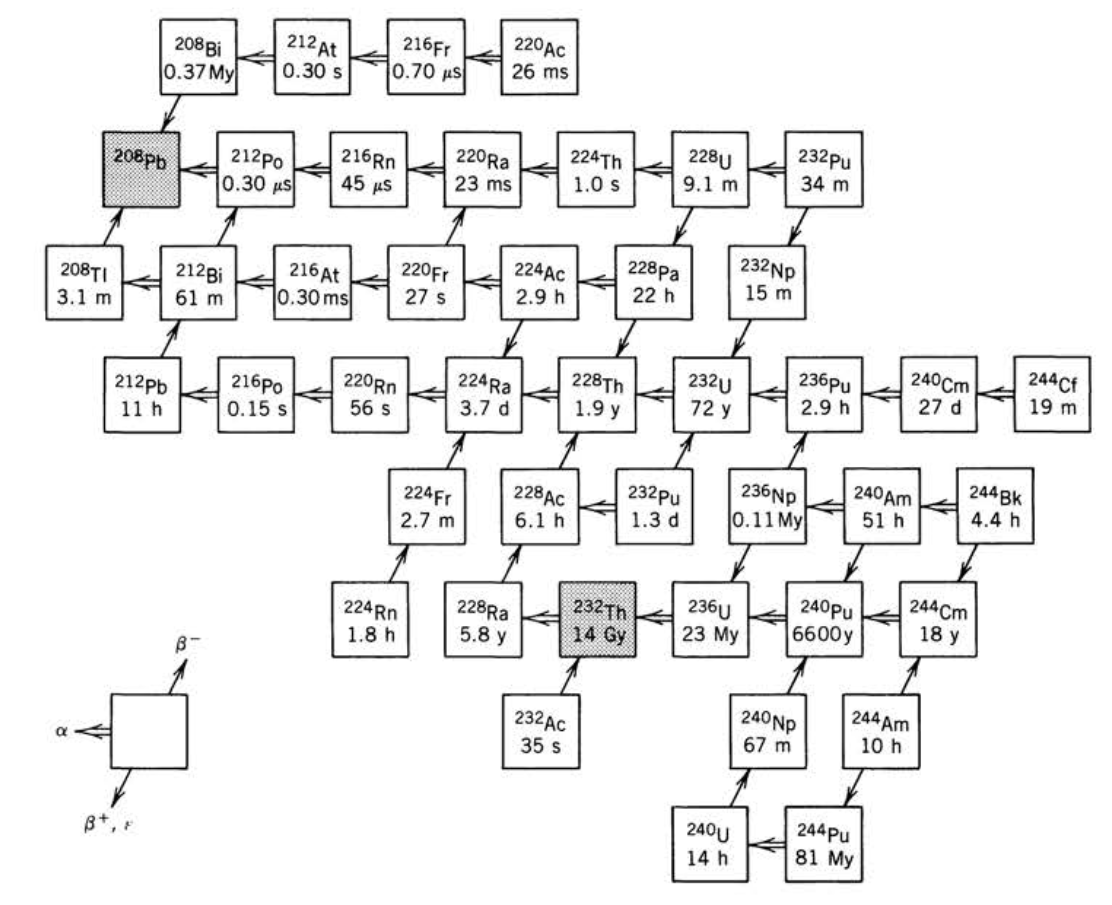
\includegraphics[width=0.9\linewidth]{foto/serie_torio.png}
  \caption{Serie del Torio}
  \label{fig:etichetta}
\end{figure}

% \include{chapters/capitolo_2}

% \include{chapters/capitolo_3}

% \include{chapters/capitolo_4}

% \include{chapters/capitolo_5}

% \include{chapters/capitolo_6}

% \include{chapters/capitolo_7}

% \include{chapters/capitolo_8}

% \include{chapters/capitolo_9}

% \include{chapters/capitolo_10}

% \include{chapters/capitolo_11}

% \include{chapters/capitolo_12}

% \include{chapters/capitolo_13}

% \include{chapters/capitolo_14}

% --- Esercitazioni ---
\setcounter{chapter}{0}
\renewcommand{\thechapter}{\Roman{chapter}}
\renewcommand{\theHchapter}{Es.\arabic{chapter}}
\renewcommand{\chaptername}{Esercitazione}

\newgeometry{
    a4paper,
    top=24mm,
    bottom=28mm,
    left=39mm,
    right=39mm,
    heightrounded
}
\partpage{Esercitazioni}
\restoregeometry

\chapter{Datazione}

Una delle applicazioni più note della radioattività è la datazione, cioè la misura dell'età di un campione a partire dalla sua composizione isotopica. 

L'idea di fondo è sempre la stessa: un nucleo radioattivo decade con una costante $\lambda$ fissata, che non dipende dalle condizioni esterne come temperatura o pressione. Il rapporto tra il numero di nuclei padre e il numero di nuclei figli accumulati funziona quindi da \emph{orologio}, purché si conosca la composizione del campione all'istante iniziale e purché il sistema sia rimasto chiuso, cioè non ci siano stati scambi con l'ambiente. 

La scelta dell'isotopo dipende dalla scala di tempi che si vuole misurare: l'orologio è utile finché non è passato troppo tempo rispetto alla vita media, altrimenti il nucleo padre è ormai scomparso. Per le rocce si usano quindi nuclei con vite medie dell'ordine del miliardo di anni, come gli isotopi dell'uranio, mentre per i reperti archeologici si ricorre al $^{14}\mathrm{C}$, che ha una vita media di qualche migliaio di anni.\\

\section{Datazione con U - Pb}

Andiamo a sfruttare quanto studiato sul decadimento dei nuclei per ottenere una datazione delle rocce in cui si ha una catena di decadimento $U - Pb$.

Gli isotopi dell'uranio $^{235}U$ e $^{238}U$ fanno una serie di decadimenti fino ad arrivare, rispettivamente, a $^{207}Pb$ e $^{206}Pb$, che sono atomi stabili. 
%
\begin{align}
    ^{235}U \longrightarrow  \cdots \longrightarrow \ ^{207}&Pb \qquad T_{1/2}^{235} = 7 \cdot 10^{8} \ y\\
    ^{238}U \longrightarrow  \cdots \longrightarrow \ ^{206}&Pb \qquad T_{1/2}^{238} = 4,5 \cdot 10^{9} \ y
\end{align}
L'orologio consiste nel misurare il rapporto $N_{Pb}(t)/N_{U}(t)$, dove $t = 0$ corrisponte al momento in cui l'uranio è stato creato (che corrisponde alla ``nascita'' della roccia), mentre $t$ corrisponde ad adesso.\\
Sappiamo che il numero di atomi di uranio in funzione del tempo corrisponde a 
%
\begin{equation*}
    N_{U}(t) = N_0 e^{-\lambda_U t}
\end{equation*}
Inoltre, se supponiamo che all'istante iniziale il numero di atomi di piombo sia \emph{nullo} e che il sistema sia chiuso si ha che 
%
\begin{equation}
    N_{Pb}(t) = N_0 - N_{U}(t) = N_0 (1 - e^{- \lambda_U t})
    \label{eq:numero_Pb}
\end{equation}
Quindi il rapporto tra queste due quantità risulta essere 
% 
\begin{tcolorbox}[colback=yellow!10!white, colframe=orange!70!black, boxrule=0.8pt]
\begin{equation}
    \frac{N_{Pb}(t)}{N_{U}(t)}  = e^{\lambda_U t} - 1
\end{equation}
\end{tcolorbox}
Questo risultato mi permette di ottenere la datazione di una roccia a partire dal rapporto tra $U$ e $Pb$ che trovo \emph{ora} nella roccia.\\

Dato che abbiamo due catene di decadimenti in base all'isotopo di uranio iniziale, possiamo andare a considerare due orologi. \\
Tornando alla relazione precedente, possiamo scrivere un orologio per ciascuna delle due catene e definire le due quantità
%
\begin{align}
    x & \equiv \frac{N_{Pb207}(t)}{N_{U235}(t)} = e^{\lambda_{235} t} - 1 \\
    y & \equiv \frac{N_{Pb206}(t)}{N_{U238}(t)} = e^{\lambda_{238} t} - 1
\end{align}
Se le ipotesi fatte sono corrette (sistema chiuso e assenza di piombo iniziale) i due orologi devono segnare tempi compatibili, cioè lo stesso $t$. 

Possiamo allora ricavare il tempo dal primo orologio
%
\begin{equation*}
    t = \frac{\ln(1 + x)}{\lambda_{235}}
\end{equation*}
e sostituirlo nel secondo, ottenendo una relazione che lega direttamente $x$ e $y$
%
\begin{equation*}
    y = \exp \left[ \frac{\lambda_{238}}{\lambda_{235}} \ln(1+x) \right] - 1
\end{equation*}
cioè
%
\begin{tcolorbox}[colback=yellow!10!white, colframe=orange!70!black, boxrule=0.8pt]
\begin{equation}
    y = (1 + x)^{\frac{\lambda_{238}}{\lambda_{235}}} - 1
\end{equation}
\end{tcolorbox}
Questa curva, introdotta da Wetherill, prende il nome di curva della concordia\mkeyword{curva della concordia}. 

\begin{figure}[htbp]
\centering
\begin{tikzpicture}[x=0.16cm, y=6cm]

% assi
\draw[->] (0,0) -- (58,0) node[anchor=north east] {$x$};
\draw[->] (0,0) -- (0,1.1) node[anchor=south east] {$y$};

% curva della concordia
\draw[thick, domain=0:52, samples=200, smooth] plot (\x, {pow(1+\x,0.158)-1});
\node[rotate=13] at (32,0.78) {concordia};

% retta della discordia
\draw[thick, dashed] (0,0.158) -- (50,0.960);
\node[rotate=9] at (26,0.44) {discordia};

% intersezioni
\fill (2,0.190) circle (1.5pt);
\fill (40,0.800) circle (1.5pt);

\end{tikzpicture}
\caption{Diagramma di Wetherill.}
\label{fig:concordia}
\end{figure}
Poiché $\lambda_{238} < \lambda_{235}$ l'esponente è minore di $1$ e la curva risulta crescente e concava: ogni suo punto corrisponde a una roccia di una certa età, che si legge scorrendo la curva. 

Non sempre però i dati sperimentali giacciono sulla concordia. In questo caso i punti si dispongono lungo una retta detta discordia\mkeyword{discordia}, segno che il sistema non è rimasto chiuso, ad esempio per una perdita di piombo successiva alla formazione della roccia. 

\subsection{Precisazione sul decadimento}

Prima di continuare è necessario fare una precisazione sulla relazione \eqref{eq:numero_Pb} usata nella sezione precedente. 

La catena di decadimento che porta dall'uranio al piombo non è diretta, ma passa attraverso una serie di nuclei intermedi 
%
\begin{equation*}
    {}^{238}\mathrm{U} \longrightarrow \mathrm{Th} \longrightarrow \mathrm{Pa} \longrightarrow \mathrm{U} \longrightarrow \cdots \longrightarrow {}^{206}\mathrm{Pb}
\end{equation*}
Di conseguenza la relazione $N_{Pb} = N_0 - N_U$ non è esatta, perché una parte dei nuclei iniziali si trova in uno degli stadi intermedi. Il bilancio corretto è infatti
%
\begin{equation*}
    N_0 = N_{U}(t) + \sum_i N_i(t) + N_{Pb}(t)
\end{equation*}
dove la somma è estesa a tutti i nuclei intermedi della catena, da cui
%
\begin{equation}
    N_{Pb}(t) = N_0 - N_{U}(t) - \sum_i N_i(t)
    \label{eq:bilancio_esatto}
\end{equation}
Per recuperare la relazione usata sopra sfruttiamo l'equilibrio secolare. Il capostipite ha infatti una vita media enormemente più lunga di quella di tutti i suoi discendenti
%
\begin{equation*}
    T_{1/2}({}^{238}\mathrm{U}) \gg T_{1/2}(i) \qquad \forall i
\end{equation*}
e quindi la catena si trova in equilibrio secolare, per cui tutte le attività sono uguali
%
\begin{equation*}
    \lambda_i N_i = \lambda_{238} N_{238} \qquad \Longrightarrow \qquad N_i = \frac{\lambda_{238}}{\lambda_i} N_{238}
\end{equation*}
Poiché $\lambda_i \gg \lambda_{238}$, il rapporto $\lambda_{238}/\lambda_i$ è trascurabile e con esso lo è il numero di nuclei intermedi presenti a ogni istante. La \eqref{eq:bilancio_esatto} diventa quindi 
%
\begin{tcolorbox}[colback=yellow!10!white, colframe=orange!70!black, boxrule=0.8pt]
\begin{equation}
    N_{Pb}(t) = N_0 - N_{U}(t) - \sum_i N_i(t) \simeq N_0 - N_U(t)
\end{equation}
\end{tcolorbox}
In altre parole, i nuclei intermedi funzionano da semplice canale di transito: appena si formano decadono, e in ogni istante ce n'è una quantità trascurabile rispetto a $N_0$.

\newpage

\section{Datazione con $^{14}C$}

Il metodo del $^{14}C$, o metodo del radiocarbonio, è un metodo di datazione di materiale organico basato sulla misura delle abbondanze relative del $^{14}C$, un isotopo radioattivo del carbonio.\\
Il decadimento di questo isotopo di carbonio è 
%
\begin{equation}
    ^{14}C \to \ ^{14}N + e^- + \bar{\nu}
\end{equation}

Il carbonio-14 è presente nell'atmosfera perché viene continuamente prodotto dai raggi cosmici, che interagendo con i nuclei dell'aria generano neutroni; questi, catturati dall'azoto, danno luogo alla reazione
%
\begin{equation*}
    {}^{14}\mathrm{N} + n \longrightarrow {}^{14}\mathrm{C} + p
\end{equation*}
Dall'atmosfera, poi, passa alla biosfera. 

Finché l'organismo è vivo continua a scambiare carbonio con l'ambiente, attraverso la respirazione e l'alimentazione, e mantiene quindi un rapporto isotopico pari a quello atmosferico. Consideriamo allora il rapporto
%
\begin{equation}
    R_0 = \left. \frac{{}^{14}\mathrm{C}}{{}^{12}\mathrm{C}} \right|_{\text{atm}}
\end{equation}
che è il valore presente nell'atmosfera, e quindi nell'organismo, subito prima della morte. 

Alla morte lo scambio si interrompe: il $^{12}\mathrm{C}$ resta costante, mentre il $^{14}\mathrm{C}$ decade senza più essere rimpiazzato. Il rapporto misurato oggi vale quindi
%
\begin{equation}
    R(t) = \frac{N_{14}(t)}{N_{12}(t)} = \frac{N_{14}(0) e^{-\lambda_{14} t}}{N_{12}(0)} = R_0 \, e^{-\lambda_{14} t}
\end{equation}
dove $t = 0$ è il momento in cui l'organismo che vogliamo datare è morto. Invertendo si ottiene l'età del reperto
%
\begin{tcolorbox}[colback=yellow!10!white, colframe=orange!70!black, boxrule=0.8pt]
\begin{equation}
    t = \frac{1}{\lambda_{14}} \ln \left( \frac{R_0}{R(t)} \right)
\end{equation}
\end{tcolorbox}

\subsection{Calibrazione}

Il problema di questo metodo è che $R_0$ \emph{non è costante nel tempo}: la produzione di $^{14}\mathrm{C}$ dipende dal flusso di raggi cosmici, che varia con l'attività solare e con il campo magnetico terrestre. Per usare la tecnica serve quindi una calibrazione. 

Un modo è considerare gli anelli degli alberi: ogni anello corrisponde a un anno noto con certezza e conserva il carbonio fissato in quell'anno, per cui misurandone il $^{14}\mathrm{C}$ si ricostruisce $R_0$ anno per anno\footnote{Questa tecnica prende il nome di dendrocronologia e permette di risalire indietro di diverse migliaia di anni; per epoche più remote si usano altri archivi, come i coralli o le stalagmiti.}. 

Si costruisce così una curva di calibrazione che lega l'età ricavata dal decadimento (\emph{radiocarbon age}) all'anno di calendario. Se $R_0$ fosse davvero costante la curva sarebbe una retta, mentre quella reale oscilla attorno a questo andamento ideale. 

\begin{figure}[h]
  \centering
  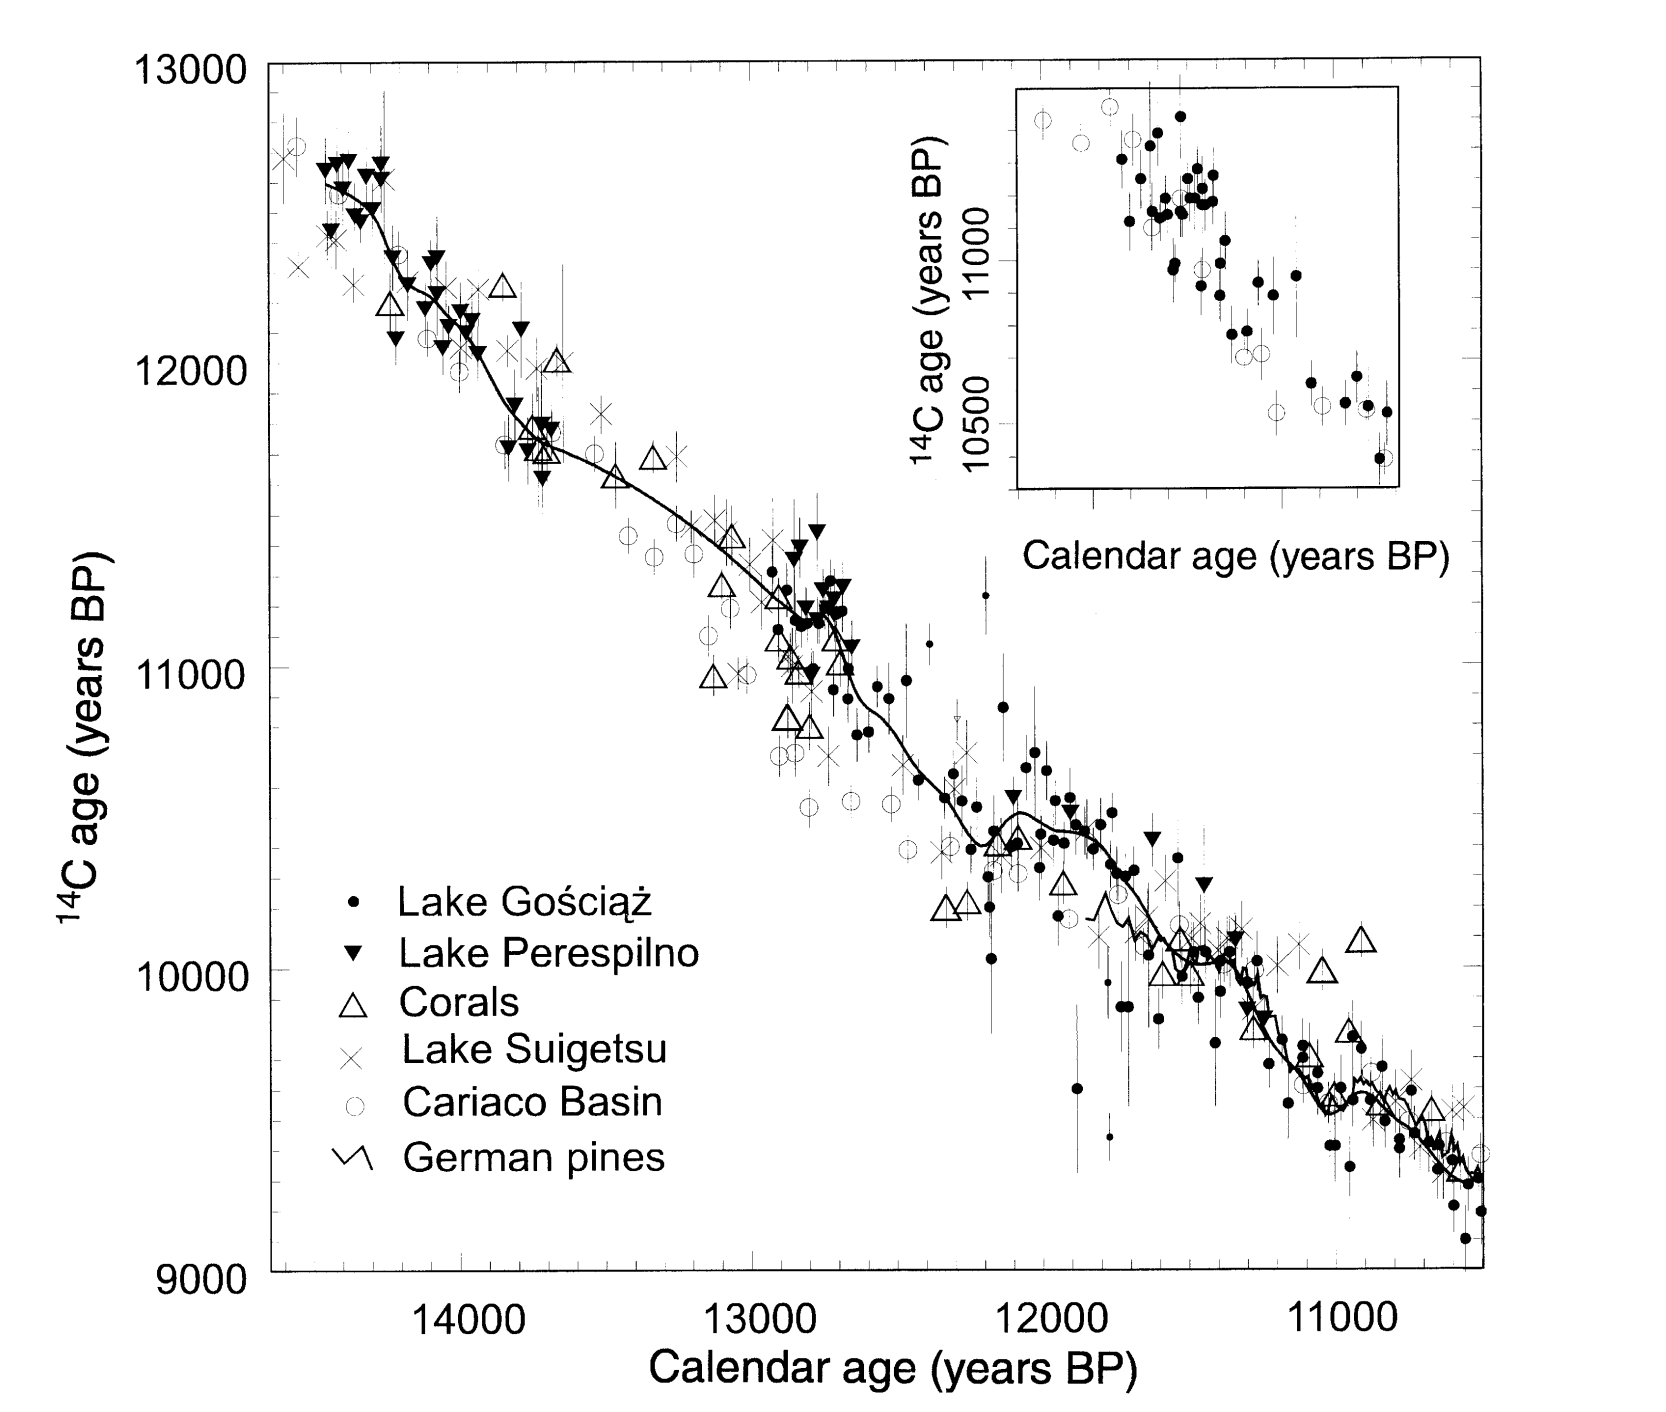
\includegraphics[width=0.75\linewidth]{foto/Radiocarbonage.png}
  \caption{Curva di calibrazione del radiocarbonio}
  \label{fig:etichetta}
\end{figure}

% \begin{figure}[htbp]
% \centering
% \begin{tikzpicture}[x=0.11cm, y=0.055cm]

% % assi
% \draw[->] (0,0) -- (0,105) node[anchor=south west, align=left] {radiocarbon\\ age};
% \draw[->] (0,0) -- (110,0) node[anchor=north west, align=left] {calendar\\ year};

% % curva ideale
% \draw[gray] (10,95) -- (100,8);
% \node[gray, anchor=north west] at (72,28) {ideale};

% % curva reale
% \draw[thick, smooth] plot coordinates {
%     (10,95) (16,72) (22,78) (28,74) (34,58) (40,52) (46,56) (52,48)
%     (58,25) (61,24) (64,58) (67,57) (70,30) (76,32) (82,20) (88,18) (94,10) (100,8)
% };
% \node[anchor=west] at (66,64) {reale};

% % lettura di una data
% \draw[dashed, gray] (0,95) -- (10,95);
% \draw[dashed, gray] (10,95) -- (10,0);
% \node[anchor=east] at (0,95) {$t$};

% \end{tikzpicture}
% \caption{Curva di calibrazione del radiocarbonio.}
% \label{fig:calibrazione}
% \end{figure}

Il fatto che la curva reale non sia monotòna è un limite intrinseco del metodo: a una stessa età radiometrica possono corrispondere più anni di calendario, e la datazione non può quindi essere resa arbitrariamente precisa. 

Inoltre la curva va corretta tenendo conto degli effetti antropici che hanno alterato il rapporto isotopico atmosferico, come l'immissione di carbonio fossile, privo di $^{14}\mathrm{C}$, e i test nucleari atmosferici degli anni Cinquanta e Sessanta, che ne hanno invece raddoppiato la concentrazione.

\end{document}